\subsubsection{Approccio Value Iteration}
Questo primo approccio di risoluzione tramite programmazione dinamica dell MDP si basa sulla costruzione, iterazione dopo
iterazione, di una value function $V_k$ che convergerà a $V^*$:
\begin{itemize}
    \item per \textbf{k = 0}: $V_0(s) = 0$  $\forall s$
    \item per \textbf{k > 0}: $V_{k+1}(s) \leftarrow \max_{a}\underbrace{\sum_{s'} P(s'|s,a)[R(s,a,s') + \gamma V_k(s')]}_{Q(s,a)}$
\end{itemize}
Quell'ultima operazione viene detta \textbf{Bellman Update} e l'operatore $\rightarrow$ è detta \textbf{Operatore di Bellman}.
La risoluzione del problema avviene calcolando ad ogni iterazione la value function che \textbf{monotonicamente convergerà} a
$V^*$. Quindi, ad una certa iterazione, se $V_k$ soddisfa il \textbf{test di convergenza} allora abbiamo trovato la value function.\\

\tikzstyle{startstop} = [rectangle, rounded corners, minimum width=3cm, minimum height=1cm, text centered, draw=black, fill=red!30]
\tikzstyle{process} = [rectangle, minimum width=3cm, minimum height=1cm, text centered, draw=black, fill=blue!30]
\tikzstyle{decision} = [diamond, aspect=2, minimum width=2cm, minimum height=0.5cm, text centered, draw=black, fill=green!30]
\tikzstyle{arrow} = [thick,->,>=stealth]


\begin{center}
    \begin{tikzpicture}[node distance=2cm]

        % Nodes
        \node (start) [startstop] {$k \rightarrow 0$,  $V_0(s) = 0, \forall s$};
        \node (iterate) [process, below of=start] {
        \begin{minipage}{4cm}
            $k \leftarrow k + 1$\\
            $\forall a, s: \text{ Calcola }Q(s, a)$
        \end{minipage}};
        \node (update) [process, below of=iterate] {Aggiorna $V_k(s) = \max_a Q(s, a)$};
        \node (check) [decision, below of=update, yshift=-0.5cm] {Convergenza?};
        \node (end) [startstop, below of=check, yshift=-2cm] {$\pi(s) = \arg\max_a Q(s, a)$};
        %\node (repeat) [process, left of=check, xshift=-4cm] {Ripeti per il prossimo stato};%
        
        % Arrows
        \draw [arrow] (start) -- (iterate);
        \draw [arrow] (iterate) -- (update);
        \draw [arrow] (update) -- (check);
        \draw [arrow] (check.south) -- ++(0,-2) node[midway, right] {Sì} -- (end.north);
        \draw [arrow] (check.west) -- ++(-2,0) node[midway, above] {No} -- ++(0,4.5) -- (iterate.west);
        %\draw [arrow] (repeat.north) |- (iterate.west);
        
        \end{tikzpicture}
\end{center}

Il \textbf{Test di Convergenza} possiamo implementarlo come la condizione:
\begin{equation}
    |\max_s \{V_{k+1}(s) - V_k(s)\} - \min_s \{V_{k+1}(s) - V_k(s)\}| \leq \varepsilon
\end{equation}
Ossia \textit{lo span (differenza tra val massimo e minimo tra i $V_k$ di 2 iterazioni dev'essere meno di un epsilon)}, oppure:
\begin{equation}
    \sum_{s} |V_{k+1} (s) - V_k(s)| \leq \varepsilon
\end{equation} 
Ossia \textit{la somma delle differenze tra i value function tra 2 iterazioni dev'essere meno di epsilon}.
Sebbene quest'algoritmo sia efficace (dimostreremo dopo perchè), non sempre è efficiente, perchè $V_k$ potrebbe \textbf{convergere lentamente}.


\subsubsection{Dimostrazione di Convergenza}
Osservando l'operatore di Bellman:
\begin{equation}
    V_{k+1}(s) \leftarrow \max_{a} \sum_{s'} P(s'|s,a)[R(s,a,s') + \gamma V_k(s')]
\end{equation}
Possiamo accorgerci di una grande somiglianza con i \textbf{giochi stocastici} e, ancora meglio, con \textbf{Expectimax} (dal momento
che quell'algoritmo puntava a massimizzare il valore atteso del reward di ogni mossa). Possiamo ricondurre un MDP ad un \textbf{gioco
stocastico ad 1 giocatore MAX}. Quindi possiamo dire che calcolare $V_k(s)$ corrisponde a risolvere un gioco stocastico di livello $k$.
Tra l'albero di gioco a profondità $k$ e $k + 1$ possiamo visualizzare questa relazione:
\begin{center}
    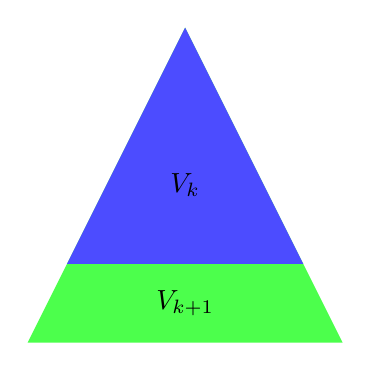
\begin{tikzpicture}

        % Triangolo verde (più grande)
        \fill[green!70] (0,0) -- (2,4) -- (4,0) -- cycle;
        
        % Triangolo blu (più piccolo e innestato)
        \fill[blue!70] (0.5,1) -- (2,4) -- (3.5,1) -- cycle;
        
        % Etichette (opzionale)
        \node at (2,2) {$V_k$};
        \node at (2,0.5) {$V_{k+1}$};
        
        \end{tikzpicture} 
\end{center}
Inoltre possiamo vedere l'albero $V_k$ come un albero di altezza $k + 1$ che ha nell'ultimo livello ($k+1$) i reward tutti nulli,
per cui $V_k$ e $V_{k+1}$ differiscono solo per i reward che all'ultimo livello sono (o potrebbero essere) $\neq 0$.\\
Sappiamo che un qualsiasi Reward $R$ è limitato:
\begin{equation*}
    R_{min} \leq R \leq R_{max}
\end{equation*}
Dunque i casi possibili sono 2:
\paragraph{Caso Migliore}Ogni reward $R = R_{max}$, per cui $V_{k+1}(s) = V_k(s) + \gamma^k R_{max}$
\paragraph{Caso Peggiore}Ogni reward $R = R_{min}$, per cui $V_{k+1}(s) = V_k(s) + \gamma^k R_{min}$
Allora un qualsiasi reward sarà sempre tra il caso migliore e il caso peggiore:
\begin{equation}
    V_k + \gamma^k R_{min} \leq V_{k+1} \leq V_k + \gamma^k R_{max}
\end{equation}
Ora facendo tendere $k \rightarrow +\infty$ otteniamo:
\begin{equation}
    V_k + 0 \leq V_{k+1} \leq V_k + 0
\end{equation}
Ossia, $V_k$ non cambia dunque abbiamo trovato una soluzione all'equazione di Bellman e che sarà necessariamente ottima.